\section{Methods}

\subsection{Overview}

\begin{figure}
    \centering
    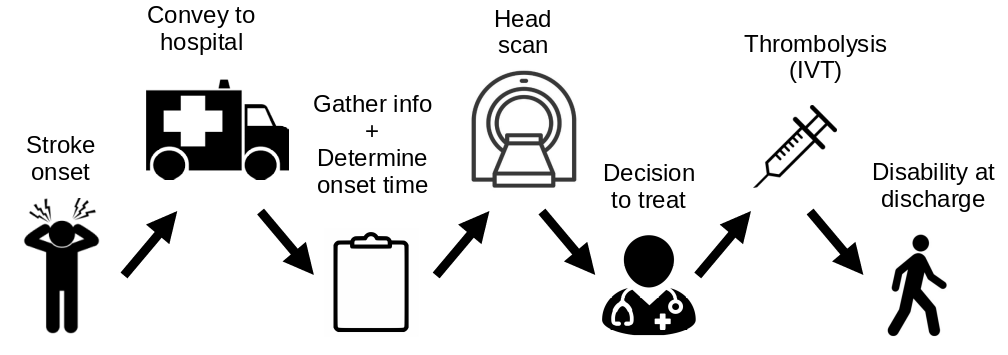
\includegraphics[width=1.0\linewidth]{images/flow}
    \caption{An overview of the process steps included in the modelling.}
    \label{fig:flow}
\end{figure}

Figure \ref{fig:flow} shows an overview of the process steps included in the modelling. Process flow was modelled by sampling from distributions of historic flow for each stroke team. Decision-making (choice of thrombolysis) was modelled with machine learning, learning which patients would likely be given thrombolysis at each stroke team. Outcomes were predicted using either mathematical models based on clinical trials (for the full pathway model), or clinical outcome machine learning models (for the more detailed analysis of differences in thrombolysis decision-making between teams).

\subsection{Data}

Data was used for all emergency stroke admissions to England and Wales for the 5 years 2017-2021, extracted from the national stroke registry for England, Wales and Northern Ireland, the Sentinel Stroke National Audit Programme (SSNAP). The registry contains all consecutive patients admitted to 100\% of acutely-admitting hospitals with a case ascertainment of over 90\% when compared to administrative data (Hospital Episode Statistics). Data was retrieved for teams with at least 250 admissions over the 5 years. The total number of patients was 302,715, of whom 114,625 (38\%) arrived within 4 hours of known stroke onset. Of those arriving within 4 hours of known stroke onset 103,244 (90\%) arrived by ambulance.

The following data fields from SSNAP were used in the modelling:

\begin{itemize}

    \item \textit{Stroke team}: Stroke team attended (hospital identifier).

    \item \textit{Age}: As midpoint of 5 year age bands.

    \item \textit{Sex}: Sex of patient (male/female)

    \item \textit{Diagnosis of atrial fibrillation}: Did the patient have a diagnosis of atrial fibrillation, either made prior to admission, or during admission?

    \item \textit{Use of anticoagulants}: Use of prior anticoagulant for atrial fibrillation.

    \item \textit{Onset known}: Whether onset was known, and if known whether it was considered to be known precisely or was a best estimate.

    \item \textit{Onset during sleep}: Did stroke occur in sleep? (1 = Yes, 0 = No).

    \item \textit{Onset-to-arrival time}: Time from onset of stroke to arrival at hospital (minutes), when known.

    \item \textit{Prior disability level}: Estimated modified Rankin Scale, mRS, prior to stroke.

    \item \textit{Stroke type}: Infarction/haemorrhage.

    \item \textit{Stroke severity}: National Institutes of Health Stroke Scale (NIHSS) score on arrival.

    \item \textit{Arrival-to-scan time}: Time from arrival at hospital to scan (minutes), when known.

    \item \textit{Scan-to-thrombolysis time}: Time from arrival at hospital to scan to treatment with thrombolysis  (minutes), when given.

    \item \textit{Disability on discharge}: mRS (0-6) on discharge, includes death (mRS 6) during admission.
    
\end{itemize}


\subsection{Thrombolysis decision model}

The thrombolysis decision model has been described in more detail previously \cite{pearn_what_2023}. Feature selection was used to identify 10 key features that were most predictive of whether thrombolysis was used in any given stroke team. The model uses XGBoost \cite{chen_xgboost_2016} for predictions, and SHAP \cite{lundberg_unified_2017} for local (patient-level) and global (model/population-level) explainability. SHAP values show the contribution of each feature value to the final model predictions.

The thrombolysis decision model was applied only to patients arriving within 4 hours of known stroke onset (stroke onset was known precisely or was a best estimate). The 10 features used for predicting thrombolysis use were: Stroke team; Age; Precisely known onset time; Onset during sleep; Onset-to-arrival time; Arrival-to-scan time; Stroke type; Stroke severity; Prior disability level; Use of anticoagulants.

Code, with demonstration, is available \cite{allen_samuel_code_2024}.

\subsubsection{Prototype patients}

To help compare decision-making and outcomes across stroke teams we exemplified differences using \textit{prototype patients}. These prototype patients captured a range of features known to affect decisions to treat, and to affect outcomes, and included an \textit{ideal} candidate for thrombolysis. The prototype patients used were:

\begin{enumerate}
    \item \textit{Ideal}: Onset-to-arrival = 90 minutes; arrival-to-scan = 15 minutes; onset-to-thrombolysis = 120 minutes; stroke severity (NIHSS) = 15; pre-stroke disability (mRS) = 0; age = 72.5; precisely known onset; onset not during sleep; stroke type = infarction; patient has no atrial fibrillation and is not receiving anticoagulants for atrial fibrillation.

    \item \textit{Late arrival}: As \textit{ideal} but onset-to-arrival = 225 minutes and onset-to-thrombolysis (when given) = 255 minutes.

    \item \textit{Mild}: As \textit{ideal} but stroke severity = 3.

    \item \textit{Prior disability}: As \textit{ideal} but pre-stroke disability = 3

    \item \textit{Imprecise}: As \textit{ideal} but stroke onset time estimated.

    \item \textit{Age}: As \textit{ideal} but age = 87.5.

    \item Combinations of the above.
\end{enumerate}

\subsubsection{Benchmark stroke teams and benchmark decisions}

SHAP isolates the contributes of features to model predictions. As one feature is the stroke team, the stroke team SHAP shows the influence of attending that stroke team on the likelihood of a patient receiving thrombolysis. Averaging stroke team SHAP values for all patients attending a given hospital provided a measure of the overall willingness of that stroke team to use thrombolysis (or how much that stroke team affected the odds of a patient receiving thrombolysis in the model). We took the stroke teams with the 25 highest stroke team SHAP values as \textit{benchmark stroke teams}. For any given patient, predictions can be made about whether each of the stroke teams would, or would not, give that patient thrombolysis. We took a majority vote of those 25 decisions as a \textit{benchmark decision} for that patient.

\subsection{Stroke outcome machine learning model}

The machine learning model predicting disability/death at discharge (mRS) is described in more detail in a companion paper \cite{pearn_are_2024}. Briefly, we used XGBoost \cite{chen_xgboost_2016} to predict outcome (mRS level) based on the following features:

\begin{enumerate}
    \item \textit{Prior disability level}: Disability level (mRS) before stroke
    \item \textit{Stroke severity}: Stroke severity (NIHSS) on arrival
    \item \textit{Stroke team}: Attended hospital
    \item \textit{Age}: Age (as middle of 5 year age bands)
    \item \textit{Onset to thrombolysis time}: Time from onset to receiving thrombolysis (minutes). Set to 9999 if did not receive thrombolysis.
    \item \textit{Any afib diagnosis}: Patient has a diagnosis of atrial fibrillation (either on arrival or new)
    \item \textit{Precise onset known}: Onset time recorded is precise time (not a best estimate)
\end{enumerate}

\subsection{Mild stroke}

We used the machine learning and decision models to specifically investigate the expected benefit or harm from mild stroke (NIHSS 0-4) in three groups: 1) All admissions within 4 hours of stroke onset, 2) Patients who had received thrombolysis, 3) Patients where the \textit{benchmark decision} would be to give thrombolysis.

\subsection{Lifetime economic model}

Data about further admissions and mortality was provided for acute stroke patients discharged between 2013 and 2014 from a large English service.  This was combined with data from UK life tables to create a set of parametric equations in a model that use age, sex, and modified Rankin Scores to predict the life-time risk of mortality and secondary care resource utilisation including Emergency Department attendances, non-elective admissions, and elective admissions. A cohort of 1,509 (male 51\%; mean age 74) stroke patients had median follow-up of seven years and represented 7,111 post-discharge patient years.  A logistic model estimated mortality within twelve months of discharge and a Gompertz model was used over the remainder of the lifetime. Hospital attendances were modelled using a Weibull distribution. Non-elective and elective bed days were both modelled using a log-logistic distribution. Assumed utiltites by mRS at discharge were based on values reported by Dijkland \textit{et al}. \cite{dijkland_utility-weighted_2018}. The lifetime economic model is described in detail by McMeekin \textit{et al}. \cite{mcmeekin_lifetime_2024}, and a full code for the economic model is available \cite{laws_stroke-optimiststreamlit_lifetime_stroke_2024}.

\subsection{Pathway model}

The pathway model has been described in more detail previously \cite{allen_use_2022}, though has been extended here to model changes in the pre-hospital pathway (ambulance response). Briefly, we model processes, including variation, using a Monte Carlo simulation model of the clinical pathway. This samples onset-to-arrival times, process times, determination of stroke onset time, and decision to thrombolyse from distributions based on historic data for each stroke team. The model predicts thrombolysis use and times for a year's admission to each stroke team (100 replicates are run, simulating 100 years admissions). Clinical outcome is predicted as the number of \textit{good outcomes} (mRS 0-1) per 1,000 admissions using a previously described mathematical model \cite{allen_estimation_2020}.

The pathway model may be used to examine a range of possible changes to improve use and speed of thrombolysis:

\begin{enumerate}

    \item \textit{Base}: Uses the hospitals’ recorded pathway statistics.

    \item \textit{Speed}: Sets 95\% of patients having a scan within 4 hours of arrival, and all patients have 15 minutes arrival-to-scan time and 15 minutes scan-to-needle time.

    \item \textit{Ambo}: Subtracts 15 minutes from the current ambulance call to arrival-at-hospital times.

    \item  \textit{Onset-known}: Sets the proportion of patients with a known stroke onset time to the national upper quartile if currently less than the national upper quartile.

    \item \textit{Benchmark}: The benchmark thrombolysis rate takes the likelihood to give thrombolysis for patients scanned within 4 hours of onset from the majority vote of the 25 benchmark hospitals (see above).

    \item Combinations of the above.
    
\end{enumerate}

Code, with demonstration, is available \cite{allen_samuel_code_2024}.